\begin{frame}{Electroweak Interaction}
    \setbeamercolor{normal text}{fg=gray,bg=}
    \setbeamercolor{alerted text}{fg=black,bg=}
    \usebeamercolor{normal text}
    \begin{columns}[T]
        \alert<1, 2>{ \begin{column}{0.5\textwidth}
            \begin{itemize}
                \item Charged Currents (CC)
                \item $W^\pm$-Boson interactions
                \begin{itemize}
                    \item left handed fermions
                    \item right handed anti-fermions
                    \item [\rightarrow] violates \textbf{C} and \textbf{P}
                \end{itemize}
                \item[] \includegraphics<2>[width=0.7\textwidth]{content/images/Wdecay1.png}
                        \includegraphics<3, 4>[width=0.7\textwidth]{content/images/Wdecay2.png}
            \end{itemize}
        \end{column}}
        %-------------%\textcolor
        \alert<3, 4>{\begin{column}{0.5\textwidth}
            \begin{itemize}
                \item Neutral Currents (NC)
                \item Z-Boson, Photon
                \begin{itemize}
                    \item decays into $l\bar{l}$
                    \item never observed: $Z \rightarrow e^{\pm} \mu^{\mp}$
                \end{itemize}
                \visible<4>{\item[] 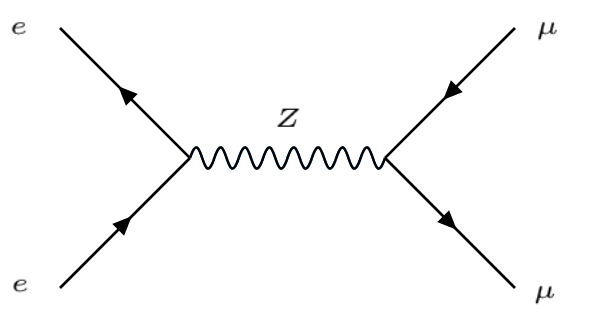
\includegraphics[width=0.8\textwidth]{content/images/Zdecay1.png}}
            \end{itemize}
        \end{column}}
    \end{columns}
\end{frame}

\begin{frame}{Charged Current \footnotemark }
    \begin{columns}
        \begin{column}{0.65\textwidth}
            In the SM, the lagrangian for the charged current is 
    \begin{equation*}
        \mathcal{L}_{CC} = \frac{g_1}{2 \sqrt{2}}  \left\{ W^{\dagger}_\mu \left[ \bar{u} \gamma^\mu (1-\gamma^5) d + \bar{\nu}_e \gamma^{\mu} (1-\gamma^5) e \right] \right\}
    \end{equation*}
    \begin{itemize}
        %\item $W^{\dagger}_{\mu} \hat{=} \text{boson field} $
        %\item $u, d \hat{=} \text{uptype, downtype quarks} $
        %\item $e \hat{=} \text{lepton}$
        %\item $\nu_e \hat{=} \text{neutrino}$
        \item $g_1 = \frac{e}{sin{(\theta_W)}}$
        \item independent of mass
    \end{itemize}
        \end{column}
        \begin{column}{0.35\textwidth}
            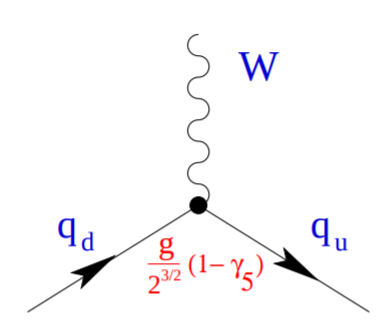
\includegraphics[width = 0.65\textwidth]{content/images/cc1.png}
            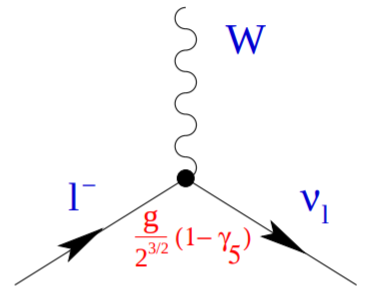
\includegraphics[width = 0.65\textwidth]{content/images/cc2.png}
        \end{column}
    \end{columns}
    \footnotetext{arXiv:hep-ph/0502010}
\end{frame}

\begin{frame}{Neutral Current}
    \begin{columns}
        \begin{column}{0.65\textwidth}
            In the SM, the lagrangian for the neutral current is 
    \begin{equation*}
        \mathcal{L}_\text{NC} = \frac{g_2}{2 \sin{(\theta_W)}} Z_\nu \sum_f \bar{f} \gamma^\mu \left( \nu_f - a_f \gamma_5 \right) f
    \end{equation*}
    \begin{itemize}
       % \item $a_f = T^f_3$
       % \item $ \nu_f = T^f_3( 1 - 4 |Q_f| \sin^2{(\theta_W)} ) $
        \item $ g_2 = \frac{e}{cos{(\theta_W)}} $
        \item independent of mass
    \end{itemize}
    \begin{figure}
        \centering
        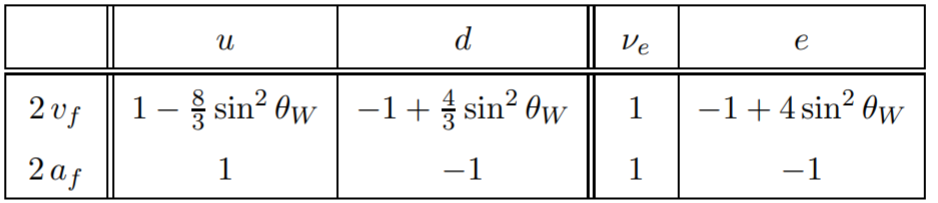
\includegraphics[width=0.8\textwidth]{content/images/nc_coublings.png}
    \end{figure}
        \end{column}
        \begin{column}{0.35\textwidth}
            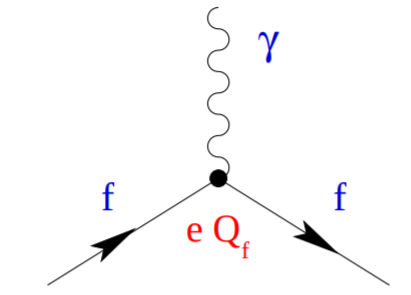
\includegraphics[width = 0.65\textwidth]{content/images/nc1.png}
            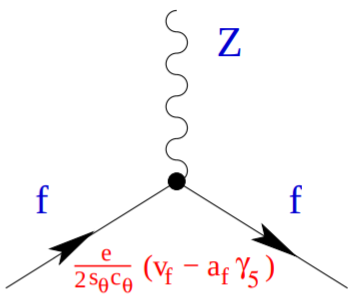
\includegraphics[width = 0.65\textwidth]{content/images/nc2.png}
        \end{column}
    \end{columns}
\end{frame}

\begin{frame}{Lepton Universality}
    \begin{itemize}
        \item charged and neutral currents studied:
        \begin{itemize}
            \item inpependent of mass
            \item constant coupling to all leptons
        \end{itemize}
        \item [\rightarrow] lepton flavour does not matter
    \end{itemize}
\end{frame}